%!TEX root = ../main.tex

\subsection{FeSO$_4$}
\label{ssec:sulfate}

Lastly, the Mössbauer spectrum of FeSO$_4$ is evaluated under the same aspects as the
previous samples. Only the results gathered from analysis will be listed here. For a
discussion of systematics and more information how the analysis is conducted earlier
sections of this lab report can be referred to. Overall, two absorption peaks are
visible in the Mössbauer spectrum of FeSO$_4$ (See \autoref{fig:sulfate} and
\autoref{tab:sulfate}).

The energetic shift of the absorption peaks caused by isomeric shift is

\begin{equation}
\Delta E = \SI{-42.74\pm 1.52e-09}{\electronvolt}.
\end{equation}

The electric field gradient is calculated as

\begin{equation}
\frac{\partial^2 V}{\partial^2 z} = \SI{9.789\pm0.517e+24}{\volt\per\meter\squared}.
\end{equation}

\begin{figure}

	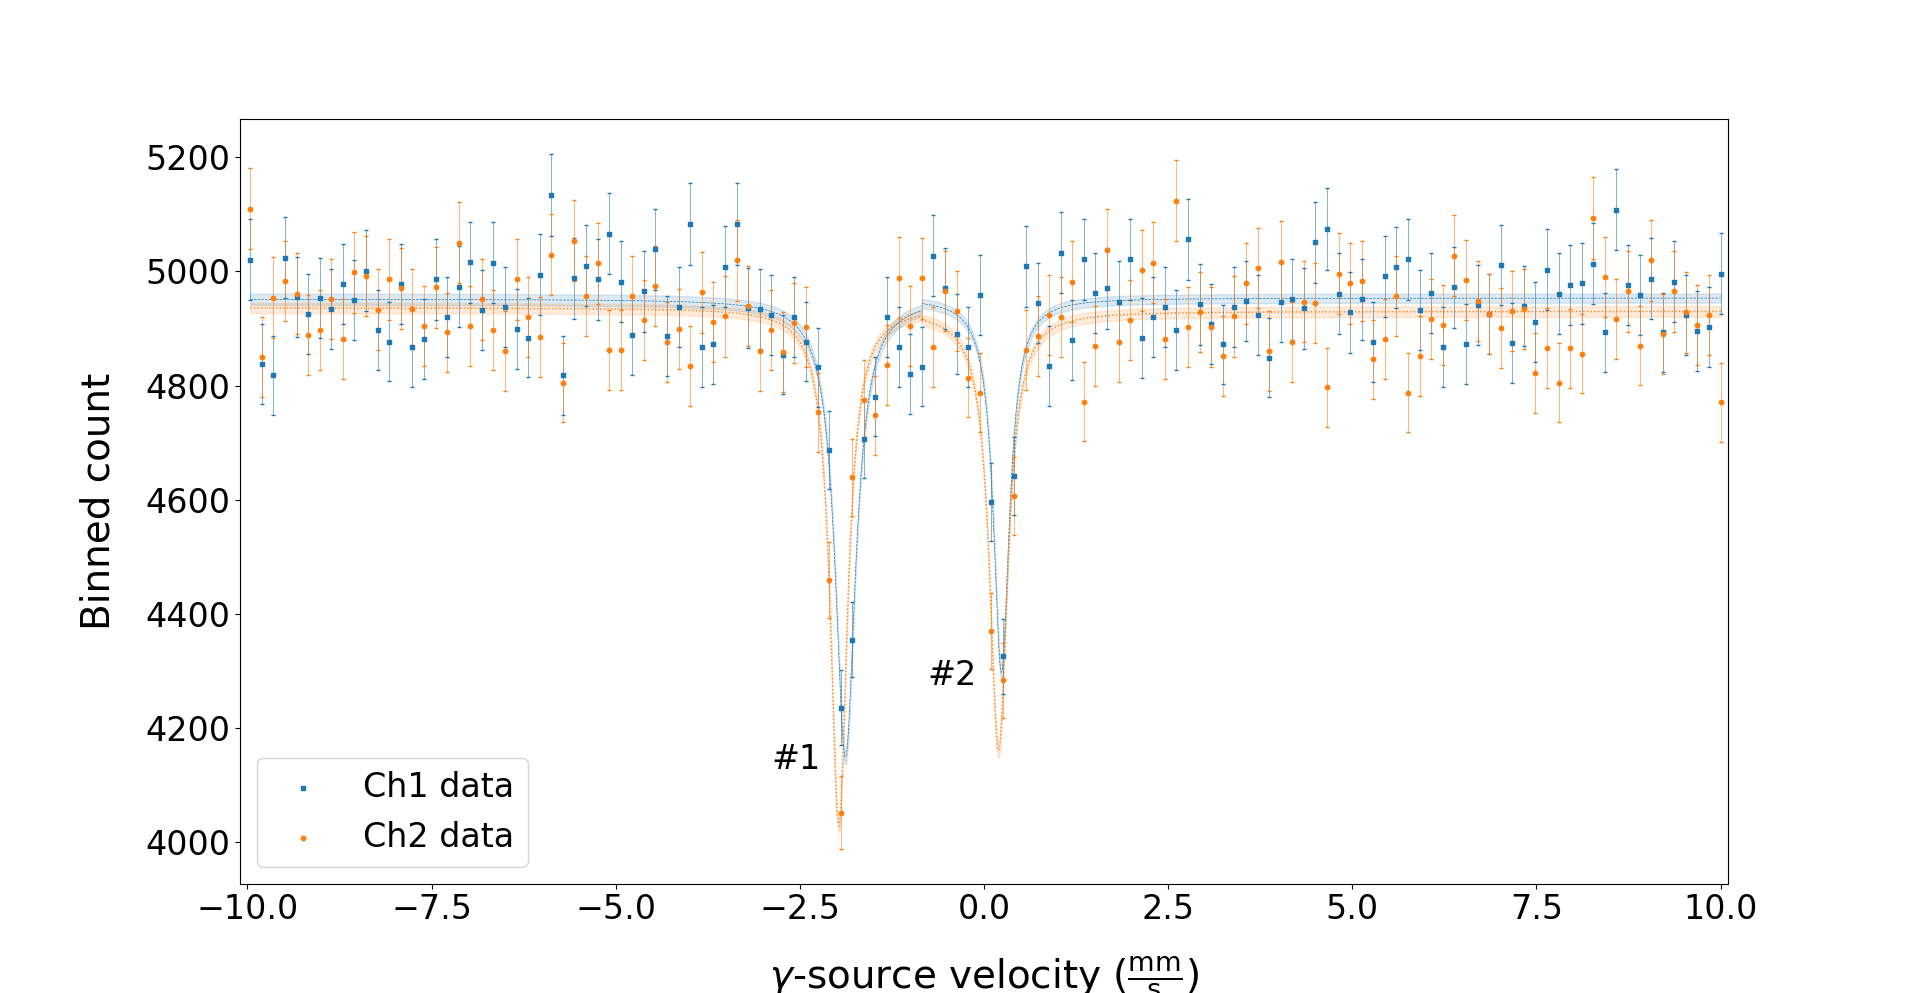
\includegraphics[width=1.0\textwidth]{./fig/Sulfate.png}
	\caption{Mössbauer spectrum of FeSO$_4$}{}
	\label{fig:sulfate}
\end{figure}

\begingroup
\renewcommand{\arraystretch}{1.3}
\begin{table}
	\begin{center}
	\caption{Mössbauer spectrum fit parameters for sulfate}
	\begin{tabular*}{0.9\textwidth}{@{\extracolsep{\fill}} c|ccccc}
  \toprule
	\hline
  Peak \# & $\Upphi_0$ & $A$ & $v_0$ & $\Gamma$ & Channel \\
	\hline
  \multirow{2}{*}{\#1} & $4951\pm10$ & $22\pm5.6$ & $-1.88\pm0.01$ & $0.334\pm0.053$ & Ch1 \\
                       & $4936\pm9$ & $18\pm3.4$ & $-1.97\pm0.01$ & $0.281\pm0.032$ & Ch2 \\
                       \hline
  \multirow{2}{*}{\#2} & $4953\pm8$ & $11\pm3.0$ & $0.24\pm0.02$ & $0.264\pm0.041$ & Ch1 \\
                       & $4930\pm9$ & $17\pm5.0$ & $0.20\pm0.01$ & $0.299\pm0.057$ & Ch2 \\
                       \hline
    \bottomrule
		\end{tabular*}
		\label{tab:sulfate}
	\end{center}

\end{table}
\endgroup

